\subsection{M.PC.8 - Efficienza temporale}
\begin{figure}[H]
    \centering
    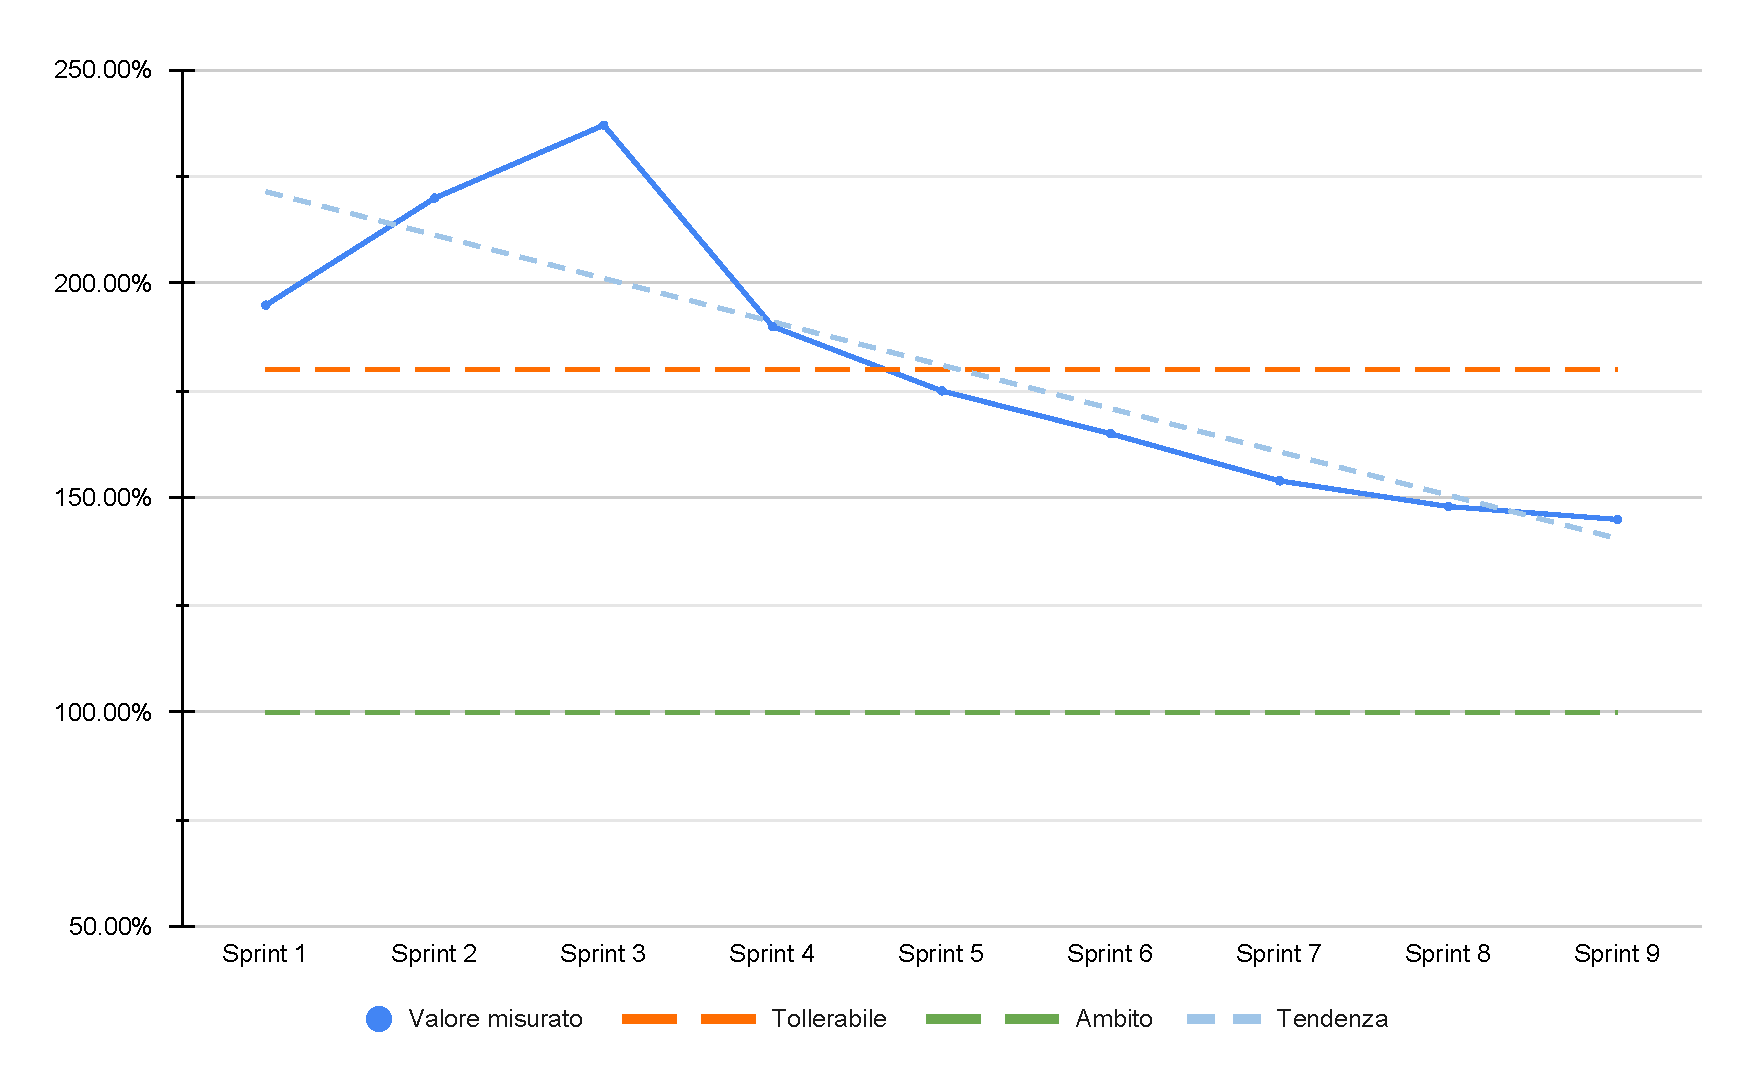
\includegraphics[width=\textwidth]{assets/efficienza_temporale.pdf}
    \caption{M.PC.8 - Efficienza temporale}
\end{figure}

\par Il grafico mostra una performance iniziale al di sotto delle aspettative, seguita da un miglioramento significativo nel corso del tempo. Nella prima fase del progetto, il gruppo ha speso un numero di ore che si è tradotto solo in minima parte in ore produttive, indicando possibili inefficienze o adattamenti necessari per la formazione e ricerca degli strumenti. Tuttavia, con il progredire degli \glossario{sprint}, si osserva un incremento costante dell'efficienza temporale. I fattori di questo miglioramento sono l'inclusione di pratiche di ottimizzazione dei processi, l'introduzione di nuovi strumenti e tecnologie, e un aumento della familiarità e della coesione del team. L'aumento dell'efficienza ha consentito al team di ridurre il valore tollerabile dal 200\% al 180\%.

\par Dopo un inizio con prestazioni inferiori alle attese, il grafico dell'efficienza temporale testimonia un percorso di miglioramento, che ha portato il team a conseguire una produttività e un ritmo apprezzabili. Questo evidenzia non soltanto una crescita in termini di rendimento, ma dimostra soprattutto l'adattabilità e la capacità di apprendimento del gruppo nel massimizzare le risorse a disposizione. Durante la \glossario{PB}, il team ha mantenuto un'efficienza costante, contribuendo a stabilizzare la traiettoria del grafico. A partire dallo \glossario{sprint} 12, il gruppo ha migliorato ulteriormente l'efficienza temporale, avvicinandosi al valore desiderato.
